% Chapter 4 (from main tex file)
% New Trends in Research
% Author: Javier Reyes

\chapter{Application}

Once the hardware has been defined and exported in Vivado Design Suite, the provided Xilinx SDK environment can be launched from the Vivado GUI itself, or via the binary installed during Vivado installation. The SDK is based on the open-source Eclipse software core, which is well known for its workspace focus. This way, when SDK is launched from Vivado, it is automatically associated with the hardware project exported, which is part of the global project that Vivado created in the first steps of the hardware definition.

\begin{figure}[h!]
	\centering
	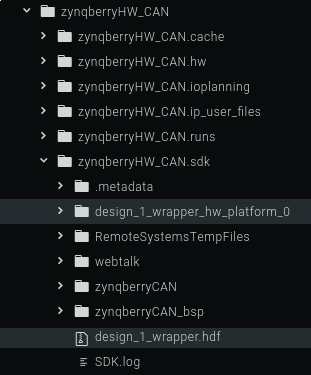
\includegraphics[width=0.5\textwidth]{xilinx-project-structure.png}
	\caption{Xilinx project structure - Hardware definition exported to SDK folder.}
	\label{fig:xilinx-project}
\end{figure}

As shown in picture \ref{fig:xilinx-project}, the SDK folder resides inside the global project created by Vivado, and the hardware export process defines both a file \texttt{.hdf} and a folder with all the correspondent information into the SDK folder (which is to be recognized as the workspace for the SDK software). Special care need to be taken with this project structure, to avoid folder or file duplicates when a change is made in the hardware definition \underline{after} the software development has been started in SDK (it is possible that the hardware gets duplicated into the SDK folder, and the software definitions are not correctly updated into the source files).

\section{Hello World application}

In order to create a software project in the Xilinx SDK environment, 

Once the SDK is ready (hardware is correctly imported), two different items need to be created in the SDK:

\begin{itemize}
	\item A Board Support Package (BSP), which contains the libraries and source files for the different modules defined in the hardware definition, correctly compiled and ready to use in a software project.
	\item A software project itself, that will use the BSP and the hardware definitions in order to create an application (either standalone, or in an embedded linux OS).
\end{itemize}

The application can be a C or C++ language-coded program, through the estandar GNU compiler colection. The SDK creates all the necessary source files (including headers) for the selected template. For a first test of the platform, a Hello World template\cite{wiki} is listed among the options. This template will provide a \texttt{helloworld.c} file, which can be renamed to a more convenient name (\texttt{main.c}).

\begin{figure}[h!]
	\centering
	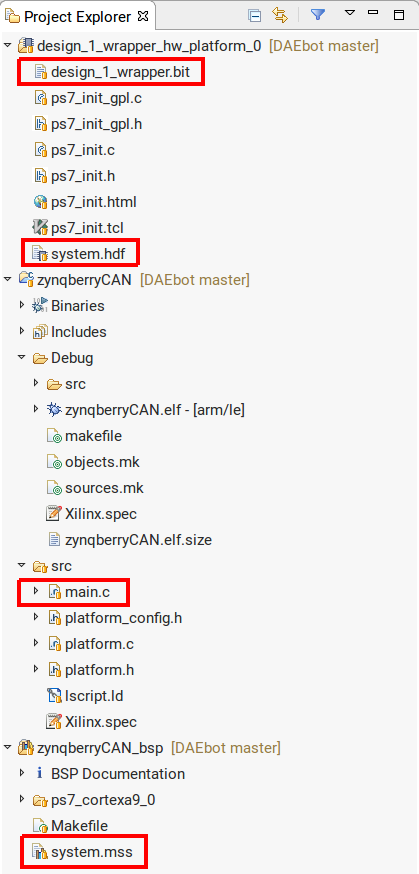
\includegraphics[width=0.4\textwidth]{sdk-projects.png}
	\caption{Xilinx SDK project structure - Relevant files.}
	\label{fig:sdk-project}
\end{figure}

The BSP need to be configured for the specific hardware platform (Zynberry board 0726), which provides a USB-to-serial converter, connected to the Zynq processor on the UART1. As the default UART defined in SDK is UART0, this setting needs to be changed. With this, the Zynq board will allow a serial communication with the host computer (via a serial console terminal program), with a baud speed of 115200 bps / 8N1 characteristics.

\begin{figure}[h!]
	\centering
	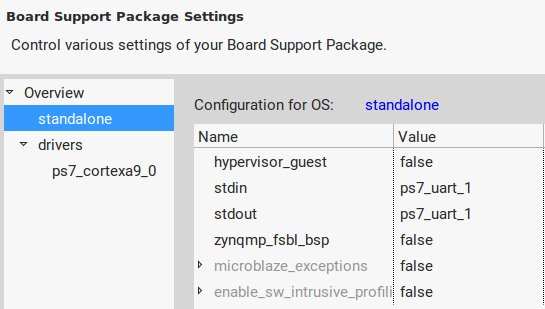
\includegraphics[width=0.6\textwidth]{bsp-std-set.png}
	\caption{BSP configuration for STDIN and STDOUT.}
	\label{fig:bsp-std-set}
\end{figure}

\section{Sensor Communication} \label{sensorcom}

In order to provide communication with the devices in the DAEbot (via CAN bus), the application requires an appropiate driver for the CAN peripheral module in the processor. This driver is created by the SDK tool when the Board Suport Package is created from the hardware project. This created driver contains all the definitions, macros, data types and function prototypes for the correct handling of the CAN module. The documentation of this peripheral driver (as well as all the other PS peripherals found in the hardware definition) are linked in the \texttt{system.mss} file, inside the BSP folder.

The CAN functionality provided by the module is quite standard (defined in \cite{can}), so that it can be used with a rather simple code. In essence, there are 3 relevant functions coded for the CAN driver:

\begin{itemize}
	\item canConfig - A subroutine that configures the functionality and baud rate of the module.
	\item sendFrame - A subroutine that triggers a CAN frame sending from a data buffer.
	\item recvFrame - A subroutine that triggers the receiving of a CAN frame into a buffer.
\end{itemize}

This functions contain the simple, register level functions provided by the BSP CAN driver, correctly adapted to the required functionality. Additional functionality can be added to the driver in the application.

The baud rate configuration for the Xilinx peripheral module works (in essence) similarly to the oficial specification. The baud rate configuration needed to achieve the established 500 kbps speed on the robot network, requires calculation an adjustment of the Time Quanta factor, and subsequently the Baud Rate Prescaler BRP, Synchronization Jump Width SJW, Time Segment 1 and Time Segment 2 (TS1-TS2). For this purposes, the equation for the registers are provided \cite[p.~580]{UG585}:

\begin{equation}
	freqBit\_Rate = \frac{ freqCAN\_REF\_CLK }{ \left( BAUD\_RATE\_PRESCALER + 1 \right) \cdot \left( 3+TS1+TS2 \right) }
\end{equation}

In order to ease the configuration, a convenient tool is provided online\footnote{See \underline{http://www.bittiming.can-wiki.info/\#XCAN}}, that helps with the calculation for the register values of different CAN modules available on the market. This was used given the fact that the recomended flow with the equations supose to asume a value and calculate the rest of them, which led to malfunctioning during the tests in the lab. With the tool, relevant design criteria were noted:
\begin{itemize}
	\item Sample Point is 87.5\% for CANopen and DeviceNet.
	\item SJW is tipically 1 for CANopen and DeviceNet.
	\item Bit time consisting of 16 Time Quanta is recommended.
\end{itemize}

The values proposed by the tool were tested, and proved succesful CAN communication, after several calculated combinations. For further changes in the DAEbot network speed, it is recomended to update the register values with help of this tool as well.

\lstinputlisting[language=C, basicstyle=\scriptsize\ttfamily, tabsize=2, commentstyle=\color{darkgray}, keywordstyle=\color{blue}, backgroundcolor=\color{lightgray}, morekeywords={\#define}, firstline=41, lastline=56, breaklines=true, numbers=left]{../../../git/DAEbot/Devices/Zynqberry_OperatorPlus/zynqberryHW_CAN/zynqberryHW_CAN.sdk/zynqberryCAN/src/main.c}

\section{Final Application}

The basic application can be represented with the activity diagram in figure \ref{fig:activity}:

\begin{figure}[h!]
	\centering
	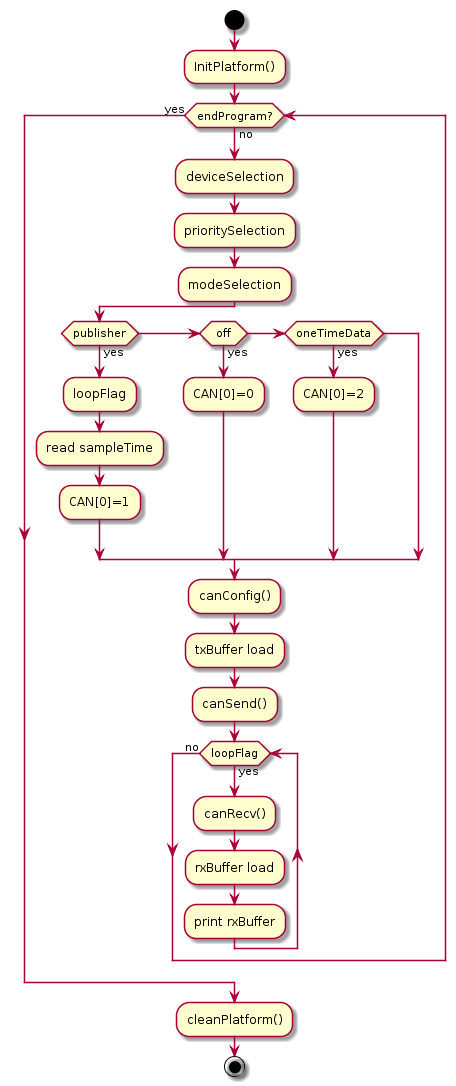
\includegraphics[width=0.5\textwidth]{activity-diag.png}
	\caption{Activity diagram for the main application for CAN connectivity.}
	\label{fig:activity}
\end{figure}

For this application to work correctly, the three functions mentioned in section \ref{sensorcom}, which will use the low level driver functions generated by the BSP.

The communication between the host computer, the Zynberry device, and any of the devices in the CAN network, can be seen in the figure \ref{fig:sequence}:

\begin{figure}[h!]
	\centering
	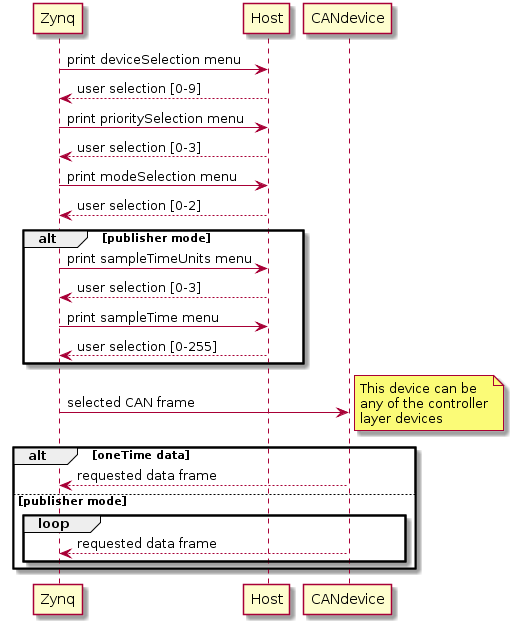
\includegraphics[width=0.6\textwidth]{sequence-diag.png}
	\caption{Sequence diagram for the main application.}
	\label{fig:sequence}
\end{figure}

At the moment of the development, only a group of devices where enabled, but further devices can be easily included in the application, by verifying that the identifier (8-bit, defined in the table available in the Wiki) is correctly located in the data array \texttt{devices}, and adding the option in the menu.

\lstinputlisting[language=C, basicstyle=\scriptsize\ttfamily, tabsize=2, commentstyle=\color{darkgray}, keywordstyle=\color{blue}, backgroundcolor=\color{lightgray}, firstline=79, lastline=91, breaklines=true, numbers=left]{../../../git/DAEbot/Devices/Zynqberry_OperatorPlus/zynqberryHW_CAN/zynqberryHW_CAN.sdk/zynqberryCAN/src/main.c}

The application running on the device, in communication with the DAEbot controllers for the available sensors can be seen as follows:

